\documentclass[11pt]{article}
\usepackage{mathtools}
\usepackage{epsfig,psfrag}
\usepackage{calligra}
\usepackage{listings}
\usepackage{color}
\usepackage{amssymb}
\usepackage[T1]{fontenc}
\usepackage[brazil]{babel}
\usepackage[sc]{mathpazo} % Use the Palatino font
\usepackage[T1]{fontenc}
\usepackage[utf8]{inputenc}
\linespread{1.05} % Line spacing - Palatino needs more space between lines
\usepackage{microtype} % Slightly tweak font spacing for aesthetics
\usepackage{algpseudocode}
\usepackage{algorithmicx}

\usepackage[hmarginratio=1:1,top=32mm,columnsep=20pt]{geometry} % Document margins
\usepackage{multicol} % Used for the two-column layout of the document
\usepackage[hang, small,labelfont=bf,up,textfont=it,up]{caption} % Custom captions under/above floats in tables or figures
\usepackage{booktabs} % Horizontal rules in tables
\usepackage{float} % Required for tables and figures in the multi-column environment - they need to be placed in specific locations with the [H] (e.g. \begin{table}[H])
\usepackage{hyperref} % For hyperlinks in the PDF

\usepackage{lettrine} % The lettrine is the first enlarged letter at the beginning of the text
\usepackage{paralist} % Used for the compactitem environment which makes bullet points with less space between them

\usepackage{abstract} % Allows abstract customization
\renewcommand{\abstractnamefont}{\normalfont\bfseries} % Set the "Abstract" text to bold
\renewcommand{\abstracttextfont}{\normalfont\small\itshape} % Set the abstract itself to small italic text

\usepackage{titlesec} % Allows customization of titles
\selectlanguage{brazil}

\usepackage{fancyhdr} % Headers and footers
\pagestyle{fancy} % All pages have headers and footers
\fancyhead{} % Blank out the default header
\fancyfoot{} % Blank out the default footer
\fancyhead[C]{{\vspace{-3cm}{\hspace{-4cm}\mbox{\begin{minipage}{1.5cm} \epsfxsize=2cm
\centerline{\epsffile{unimontes.eps}}
\end{minipage}}}{\hspace{.6cm} Computação evolutiva $\bullet$ 2015}}
} % Custom header text
\fancyfoot[RO,LE]{\thepage} % Custom footer text




%----------------------------------------------------------------------------------------
%    TITLE SECTION
%----------------------------------------------------------------------------------------

\title{\vspace{.5cm}\fontsize{24pt}{10pt}\selectfont\textbf{\sc Trabalho de otimização combinatorial com pontes rolantes}} % Article title

\author{
\large
\textsc{Herberth Amaral}\\[2mm]
\normalsize Departamento de Ciência da Computação \\
\normalsize Universidade Estadual de Montes Claros \\
\normalsize \href{mailto:herberthamaral@gmail.com}{herberthamaral@gmail.com}
\vspace{-5mm}
}
\date{\today}

%----------------------------------------------------------------------------------------

\begin{document}

\maketitle % Insert title

\begin{abstract}
    O problema das pontes rolantes é um conhecido problema de otimização
    combinatorial. Este trabalho apresenta a discussão da solução do
    problema utilizando algoritmos genéticos com um operador de mutação similar
    ao 2-opt. Os resultados mostram que a solução pode alcançar tempos da ordem
    de 8700 minutos.
\end{abstract}

\thispagestyle{fancy} % All pages have headers and footers

\newpage

\section{Introdução}
Otimização combinatorial refere-se a um campo da matemática aplicada que possui
foco em resolver problemas de otimização em estruturas discretas \cite{livro}.
Este trabalho tem como objetivo mostrar o uso de algoritmos genéticos e seus
respectivos operadores para resolver o problema das pontes rolantes.

O problema das pontes rolantes é apresentado da seguinte forma: três pontes
(nomeadamente A, B e C) em uma aciaria são responsáveis por movimentar ordens
de serviço entre os estágios de produção de aço (nomeadamente convertedor,
estação de borbulhamento, forno-panela, desgaseificação à vácuo, lingotamento
convencional e lingotamento contínuo). As principais restrições são: um estágio
não pode conter mais de uma ordem de serviço ao mesmo tempo e uma ponte não
pode "passar por cima" da outra. A ponte C possui espaço de movimentação
limitado, ficando responsável apenas por fazer movimentações entre os estágios
intermediários (forno-panela, desgaseificação à vácuo e estação de
borbulhamento) para os estágios finais (lingotamentos convecional e contínuo).
A figura \ref{fig:pontes} mostra o diagrama da aciaria.

\begin{figure}[H]
  \centering
  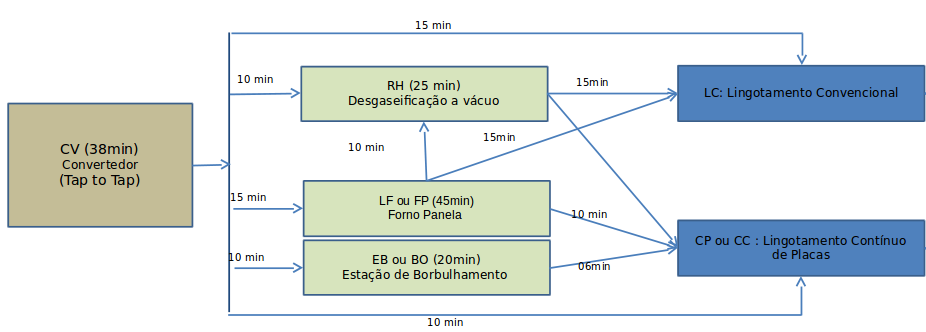
\includegraphics[width=1.0\textwidth]{pontes.png}
  \caption{Diagrama da aciaria}
  \label{fig:pontes}
\end{figure}


\section{Problema}

Como é possível ver na figura \ref{fig:pontes}, entre cada estágio há um tempo
de rota. Esse tempo de rota é diminuido pela metade se uma ponte estiver
descarregada. O principal objetivo da solução do problema é descobrir o melhor
uso das pontes de forma que o tempo de trânsito seja mínimo. O problema ainda
possui a restrição de manter a ordem de entrega das ordens de serviço, portanto
é fora de cogitação alterar a ordem de execução das ordens de seviço.

\section{Metodologia}

Para resolver esse problema, fez-se uso da meta-heurística de algoritmos
genéticos. A seguir, detalha-se a representação do indivíduo e os operadores utilizados.

\subsection{Representação do indivíduo}

Cada uma das 498 ordens de serviço tem pelo menos duas transições. Cada uma
dessas transições usa uma ponte para execução. O indivíduo, então, é
representado pelo conjunto de pontes escolhidas para executar cada uma das 1922
transições.

\subsection{Seleção}

A seleção é feita de forma aleatória dentre os 20\% da população com o melhor
fitness. Para aumentar a diversidade, o mesmo indivíduo  não é escolhido mais
de uma vez.

\subsection{Cruzamento}

O operador de cruzamento produz dois filhos e é definido da seguinte forma:
\begin{equation}
    Crossover(P_1, P_2) = 
    \begin{cases}
        P_{1i} & \quad \text{if } \mathcal{N}(0,1) > 0,5\\
        P_{2i} & \quad \text{otherwise}
    \end{cases}
    ,\forall i \in \{1\dots NumCromossomos\}
\end{equation}

O operador acima não leva em consideração a validade da solução porque considera que os pais são indivíduos válidos para o problema.

\subsection{Mutação}

O operador de mutação escolhe uma das 1922 transições e troca a ponte que será
utilizada. Esse processo necessita de cuidado porque nem toda ponte pode
executar uma determinada transição (exemplo: a ponte C não pode executar
transições de convertedores para o forno-panela).

\subsection{Parâmetros do AG}

Os seguintes parâmetros do AG foram adotados para a solução:

\begin{itemize}
    \item \textbf{População:} 100 indivíduos;
    \item \textbf{Taxa de mutação:} $0.05*\lambda$, em que $\lambda$ é o número de gerações consecutivas em que não há decaimento do melhor fitness;
    \item \textbf{Critério de parada:} 100 iterações ou $\lambda=20$;
    \item \textbf{Número de execuções:} 30.
\end{itemize}

Os tempos de processamento de cada estágio não foram considerados. Foram
considerados apenas os tempos de movimentação das pontes.

\section{Resultados}

O algoritmo genético utlizado conseguiu reduizir o tempo necessário para
processar as ordens de serviço a um mínimo de 8701 minutos. A tabela
\ref{tbl:media} mostra o decaimento médio do fitness com o passar das gerações
considerando todas as execuções.

\begin{table}[H]
    \centering
    \caption{Média das evoluções nas gerações}
    \label{tbl:media}
    \begin{tabular}{|l|l|}
    \hline
    Geração & Média ($\sigma$) \\ \hline
    0  & 9433.806 (69.1264) \\ \hline
    10 & 9208.903 (100.422) \\ \hline
    20 & 9043.903 (88.616) \\ \hline
    30 & 8984.967 (108.621) \\ \hline
    40 & 8971.741 (124.425) \\ \hline
    50 & 8963.129 (129.159) \\ \hline
    60 & 8952.225 (129.184) \\ \hline
    70 & 8948.451 (126.972) \\ \hline
    80 & 8947.580 (123.986) \\ \hline
    90 & 8947.935 (123.724) \\ \hline
    \end{tabular}
\end{table}

A figura \ref{fig:decaimento} mostra uma visualização da queda do fitness com o
passar das gerações. É interessante notar que a maior parte da queda ocorre nas
primeiras 20 gerações.

\begin{figure}[H]
  \centering
  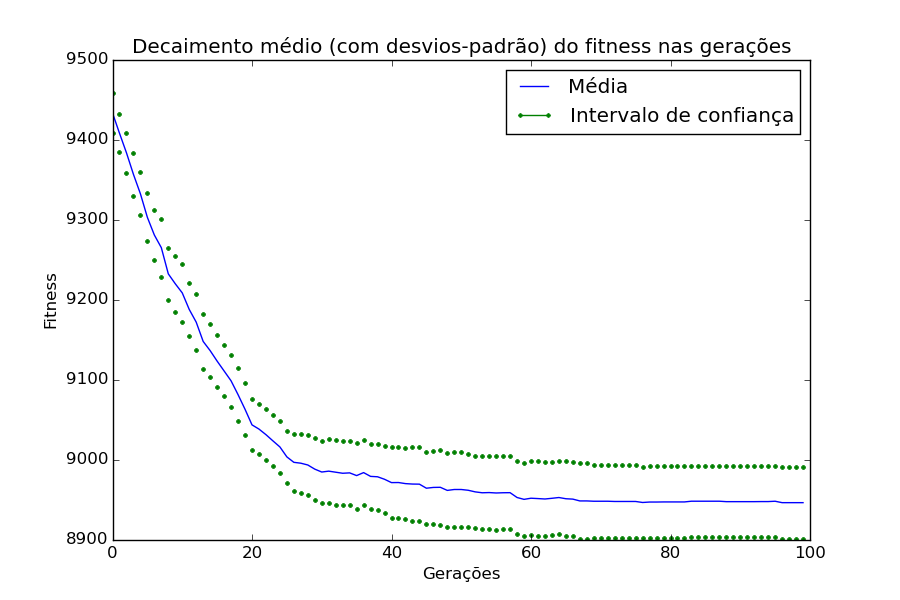
\includegraphics[width=0.7\textwidth]{decaimento.png}
  \caption{Decaimento do fitness com o passar das gerações}
  \label{fig:decaimento}
\end{figure}

O cálculo de percentis de queda podem ser usados para comprovar a afirmação
feita no parágrafo anterior. Percentis são ferramentas estatísticas úteis para
indicar um valor abaixo uma dada porcentagem de observações em um grupo de
observações. Por exemplo, o 80º percentil diz em qual geração que 80\% da
otimização foi feita. Obviamente o p100 sempre será a última geração. A tabela
\ref{tbl:percentis} mostra as gerações em que cada percentil de queda foi alcançado.

\begin{table}[H]
    \centering
    \caption{Percentis da evolução do algoritmo}
    \label{tbl:percentis}
    \begin{tabular}{|l|l|l|l|}
    \hline
    p80 & p90 & p95 & p99 \\ \hline
    11  & 16  & 19  & 21  \\ \hline
    \end{tabular}
\end{table}

Resumidamente, o que a tabela \ref{tbl:percentis} mostra é que 99\% da evolução
do algoritmo ocorre nas 21 primeiras gerações. Essa informação é importante
para uma melhor escolha do número de gerações que será escolhida.

Característica notável da implementação proposta é o baixo tempo de execução em
relação ao tempo de execução dos demais colegas de disciplina. Alguns chegaram
a reportar 17 horas de tempo de execução total em condições similares à deste
trabalho. O tempo total de execução das 30 execuções foi de 3h45m. A tabela
\ref{tbl:tempo} mostra o tempo médio e o desvio padrão de cada execução e de
cada geração:

\begin{table}[H]
    \centering
    \caption{Percentis da evolução do algoritmo}
    \label{tbl:tempo}
    \begin{tabular}{|l|l|l|l|}
    \hline
    Média de execução ($\sigma$) & Média geração ($\sigma$) \\ \hline
    456.72s (161.54s)            & 8.62s (6.16s)             \\ \hline
    \end{tabular}
\end{table}

É possível notar que os desvios padrão são bem altos proporcionalmente à média.
Isso pode ser explicado pela alta variação do número de vezes que a função
objetivo é executada em cada geração ($20 < n < 60$) para as médias da geração
e a quantidade de gerações em cada execução para o grande desvio do tempo de
execução. A tabela \ref{tbl:geracoes} permite averiguar essa afirmação.

\begin{table}[H]
    \centering
    \caption{Percentis da evolução do algoritmo}
    \label{tbl:geracoes}
    \begin{tabular}{|l|l|}
    \hline
    Execução  & Nº de gerações\\ \hline
    01 & 70 \\ \hline
    02 & 46 \\ \hline
    03 & 60 \\ \hline
    04 & 26 \\ \hline
    05 & 38 \\ \hline
    06 & 53 \\ \hline
    07 & 38 \\ \hline
    08 & 63 \\ \hline
    09 & 51 \\ \hline
    10 & 55 \\ \hline
    11 & 49 \\ \hline
    12 & 37 \\ \hline
    13 & 62 \\ \hline
    14 & 50 \\ \hline
    15 & 44 \\ \hline
    16 & 52 \\ \hline
    17 & 59 \\ \hline
    18 & 74 \\ \hline
    19 & 44 \\ \hline
    20 & 46 \\ \hline
    21 & 51 \\ \hline
    22 & 42 \\ \hline
    23 & 47 \\ \hline
    24 & 45 \\ \hline
    25 & 80 \\ \hline
    26 & 45 \\ \hline
    27 & 35 \\ \hline
    28 & 68 \\ \hline
    29 & 51 \\ \hline
    30 & 100 \\ \hline
    \end{tabular}
\end{table}

\bibliographystyle{alpha}
\bibliography{template}

\end{document}
